
\documentclass[12pt,a4paper]{article}
\usepackage[utf8]{inputenc} % sempre salve seus arquivos como UTF8
\usepackage[T1]{fontenc}
\usepackage[english]{babel}

\usepackage[left=2.5cm,right=2cm,top=2cm,bottom=2.5cm]{geometry}
\usepackage{amsmath}
\usepackage{amsthm}
\usepackage{amsfonts}
\usepackage{graphicx}
\usepackage{algorithm}
\usepackage{color}
\usepackage[noend]{algpseudocode}
\usepackage{mathtools}

% load times font
\usepackage{mathptmx}
\usepackage[scaled=.90]{helvet}
\usepackage{courier}

% comandos
\newcommand{\mdc}[1]{\mathrm{mdc}(#1)}

\DeclarePairedDelimiter\ceil{\lceil}{\rceil}
\DeclarePairedDelimiter\floor{\lfloor}{\rfloor}

% Foot without marker
\newcommand\blfootnote[1]{%
	\begingroup
	\renewcommand\thefootnote{}\footnote{#1}%
	\addtocounter{footnote}{-1}%
	\endgroup
}

\title{MO446 -- Introduction to Computer Vision  \\ Project 0}
\author{Breno Leite  \\ Guilherme Leite}
\date{10/08/2017}

\begin{document}

\maketitle
\blfootnote{\textit{\textbf{Important note:} The borders seen in the figures are not part of the image, they are figurative information about the starting and ending points of the image. Moreover, all the image scales in this report were changed in order to make the text more readable.}} \\

%% ---------------- Starts here --------------------------------

\textbf{Question 1 - Input images} \\

The Figure \ref{fig:p0-1-0} was used as an input to all the exercises, as specified it is a colored image, rectangular and its type is \emph{PNG}. Th image dimensions are 400x300, which satisfies the required size. \\

\begin{figure}[!h]
	\centering
	{%
		\setlength{\fboxsep}{1pt}%
		\setlength{\fboxrule}{1pt}%
		\fbox{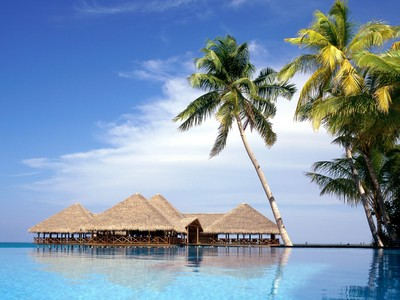
\includegraphics[scale=0.8]{input/p0-1-0}}%
	}%
	\caption{Input image used in the questions (\textbf{p0-1-0})}
	\label{fig:p0-1-0}
\end{figure}

\textit{Note:} The image was converted from \emph{JPG} to \emph{PNG} format. 

\newpage


\textbf{Question 2 - Color planes} \\

\textbf{2-a) } A PNG image is represented in RGB format, which means that there is three channels for each pixel. These channels represents the intensity of each color, in a determined pixel, RGB stands for: Red, Green, and Blue. The Figure \ref{fig:p0-2-a-0} represents an image obtained by swapping the red and blue channel in the input image.

\begin{figure}[!h]
	\centering
	{%
		\setlength{\fboxsep}{1pt}%
		\setlength{\fboxrule}{1pt}%
		\fbox{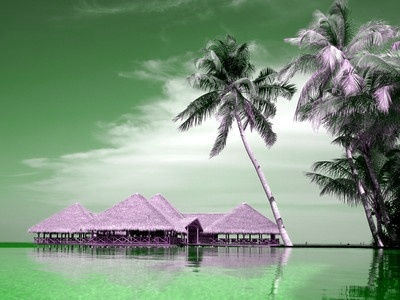
\includegraphics[scale=0.8]{output/p0-2-a-0}}%
	}%
	\caption{Input image with red and blue channels swapped (\textbf{p0-2-a-0})}
	\label{fig:p0-2-a-0}
\end{figure}

We can note a heavy intensity of green in the image after the swap, the reason for that is explained looking at the original image. Most of the pixels in the original image has a low intensity of red, in opposite, the intensity of blue is quite high mainly because of the water and sky. When the swap occurs, all the blue intensity goes to red highlighting things that had a little bit of red intensity on the original image, like the fences. \\

In other hand, all the intensity from the red (really low on the original image) goes to blue. So, that makes the intensity of blue goes down in places that blue was too high (e.g. water and sky). This way, the green color becomes more intense on places that blue was predominant on the original image, explaining the green lake.\\

\newpage


\textbf{2-b) } A monochrome or grayscale images is composed by a single channel, which ranges from 0 to 255 as RGB channels. Thus, create a monochrome image from the green channel is a straightforward procedure, it is just a copy of the green channel into a new image. The result obtained using this procedure on the input image is seen in the Figure \ref{fig:img-green}.

\begin{figure}[!h]
	\centering
	{%
		\setlength{\fboxsep}{1pt}%
		\setlength{\fboxrule}{1pt}%
		\fbox{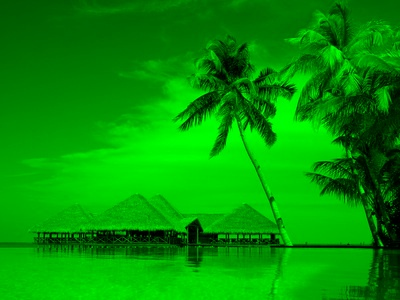
\includegraphics[scale=0.7]{output/p0-2-b-0}}%
	}%
	\caption{Monochrome image created from green channel (\textbf{p0-2-b-0})}
	\label{fig:img-green}
\end{figure}

As shown in the figure, the representation of the image stills really good. The reason for this is the high intensity of the green channel in the original image, which makes this channels, by its own, a good representation for image.\\

\textbf{2-c) } Using the same structure as in \textbf{2-c}, we this time use the red channel to create the new monochrome image, which is shown in Figure \ref{fig:img-red}.

\begin{figure}[!h]
	\centering
	{%
		\setlength{\fboxsep}{1pt}%
		\setlength{\fboxrule}{1pt}%
		\fbox{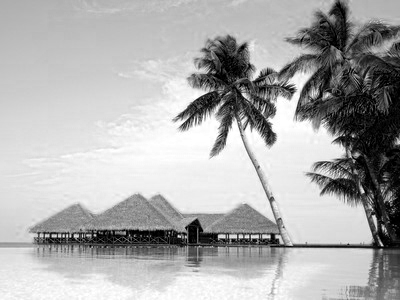
\includegraphics[scale=0.7]{output/p0-2-c-0}}%
	}%
	\caption{Monochrome image created from red channel (\textbf{p0-2-c-0})}
	\label{fig:img-red}
\end{figure}

In this image, we are able to see more blurred areas. The reason for this result is the low intensity of the red channel over the image pixels, which makes just the channel red not as good representation as the green channel.

\textbf{2-d) } The image created from the green channel (\textbf{p0-2-b-0}) looks more like what we expected, this is explained by three channels of the image. As said before, the original image is more intense on the green channel than in the red channel\footnote{Mean values for each channel in the original image: Red: 127.40, Green: 149.85, Blue: 173.02}. We normally would expect to the green approach better express the image, mainly because the nature of the green color in the real world. However, we can not expect this result for every image. \\

In contrast, we would expect to a computer work better in a image extracted from a red channel, the intuition is that the color red gives a better contrast to the image. In this way, the information like shapes of objects on the image are highlighted in the monochrome image, example are the contrast between the sky and the clouds in the Figure \ref{fig:img-red} (\textbf{p0-2-c-0}). \\

\textbf{Question 3 - Replacements of pixels} \\

In this question we merge the results shown in Figures \ref{fig:img-green} (\textbf{p0-2-b-0}) and \ref{fig:img-red} (\textbf{p0-2-c-0}). In order to do that, we inserted the centered 100x100 pixels from image \textbf{p0-2-b-0} into the image \textbf{p0-2-c-0}, the result is shown in Figure \ref{fig:p0-3-0}. 


\begin{figure}[!h]
	\centering
	{%
		\setlength{\fboxsep}{1pt}%
		\setlength{\fboxrule}{1pt}%
		\fbox{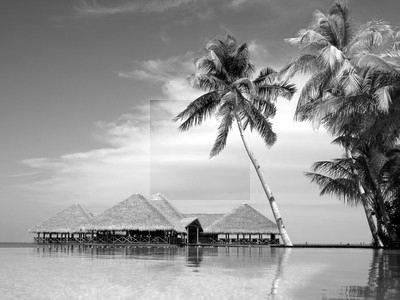
\includegraphics[scale=0.5]{output/p0-3-0}}%
	}%
	\caption{Pixels centered (100x100) from Figure \ref{fig:img-green} into Figure \ref{fig:img-red} (\textbf{p0-3-0})}
	\label{fig:p0-3-0}
\end{figure}

After that, we inserted the generated image (\textbf{p0-3-0}) into its respective channel (green) in the original image. The results is shown in Figure \ref{fig:p0-3-1}.

\begin{figure}[!h]
	\centering
	{%
		\setlength{\fboxsep}{1pt}%
		\setlength{\fboxrule}{1pt}%
		\fbox{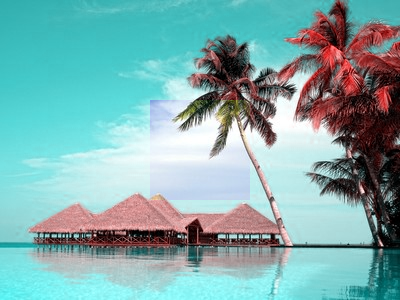
\includegraphics[scale=0.6]{output/p0-3-1}}%
	}%
	\caption{Original image with green channel replaced from Figure \ref{fig:p0-3-0} (\textbf{p0-3-1})}
	\label{fig:p0-3-1}
\end{figure}

As we can see, the image is almost the same as the original input, except by the center part. If we recall, the Figure \ref{fig:img-green} is formed by two different images. And, each of them are monochrome images created from the green and red channels of the original input. The Figure \ref{fig:channels} shows how the channels representations is represented in the Figure \ref{fig:p0-3-1}, which was created by the insertion. \\

\begin{figure}[!h]
	\centering
	{%
		\setlength{\fboxsep}{1pt}%
		\setlength{\fboxrule}{1pt}%
		\fbox{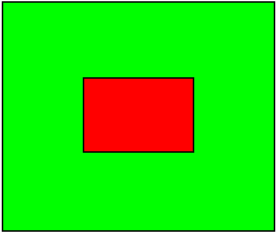
\includegraphics[scale=0.5]{report/image-color}}%
	}%
	\caption{Channels representation layout in the Figure \ref{fig:p0-3-0}}
	\label{fig:channels}
\end{figure}

When we replace the image \textbf{p0-3-0} inside the green channel of the original input, all the pixels outsize the box at the center are equal, which keeps the same pixels for all the outside-box part. In contrast, the pixels inside the box, which represents the red color, overwrites the green pixels in that region forming a different image. \\

\textbf{Question 4 - Arithmetic and geometric operations} \\

\begin{figure}[!h]
	\centering
	{%
		\setlength{\fboxsep}{1pt}%
		\setlength{\fboxrule}{1pt}%
		\fbox{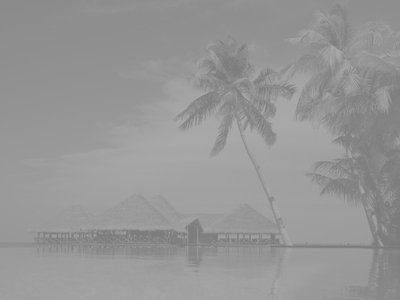
\includegraphics[scale=0.8]{output/p0-4-b-0}}%
	}%
	\caption{p0-4-b-0}
	\label{fig:p0-4-b-0}
\end{figure}


\begin{figure}[!h]
	\centering
	{%
		\setlength{\fboxsep}{1pt}%
		\setlength{\fboxrule}{1pt}%
		\fbox{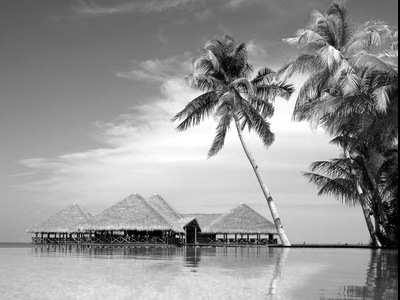
\includegraphics[scale=0.8]{output/p0-4-c-0}}%
	}%
	\caption{p0-4-c-0}
	\label{fig:p0-4-c-0}
\end{figure}

\begin{figure}[!h]
	\centering
	{%
		\setlength{\fboxsep}{1pt}%
		\setlength{\fboxrule}{1pt}%
		\fbox{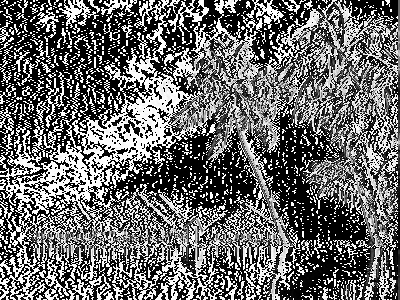
\includegraphics[scale=0.8]{output/p0-4-c-1}}%
	}%
	\caption{p0-4-c-1}
	\label{fig:p0-4-c-1}
\end{figure}

\newpage

\textbf{Question 5 - Noise} \\



\begin{figure}[!h]
	\centering
	{%
		\setlength{\fboxsep}{1pt}%
		\setlength{\fboxrule}{1pt}%
		\fbox{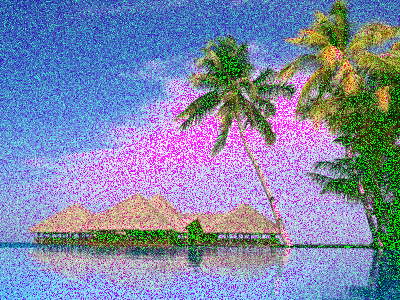
\includegraphics[scale=0.8]{output/p0-5-a-0}}%
	}%
	\caption{p0-5-a-0}
	\label{fig:p0-5-a-0}
\end{figure}

\begin{figure}[!h]
	\centering
	{%
		\setlength{\fboxsep}{1pt}%
		\setlength{\fboxrule}{1pt}%
		\fbox{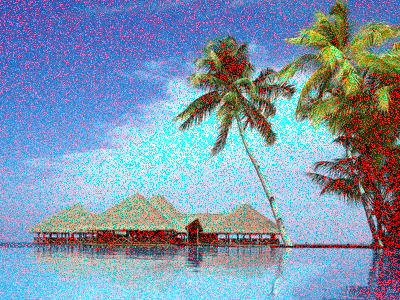
\includegraphics[scale=0.8]{output/p0-5-b-0}}%
	}%
	\caption{p0-5-b-0}
	\label{fig:p0-5-b-0}
\end{figure}


\end{document}

